\documentclass[main]{subfiles}

\begin{document}
\section{Eksperimentel Opstilling}
Delforsøg 1 og 2 har identisk opstilling på følgende punkter: En laser kilde pkt. 1 på \cref{fig:opstilling1} og \cref{fig:opstilling2} udsender en laser stråle på $\lambda \sim  \SI{900}{\nano\m} $. Herefter rammer laseren en linse, pkt. 2, der har til formål at danne en kollimeret laser stråle. Hvorefter strålens føres over i AOM'en pkt. 5, via. 2 spejle pkt 3. og en linse pkt. 4, der fokusere laser strålen i AOM'ens indgang.
\subsection{Delforsøg 1}
I dette forsøg, er AOM'en forbundet til en frekvensgenerator og en forstærker på hhv. pkt. 8 og 7 på \cref{fig:opstilling1}. Herefter bliver laser strålen diffraktions ordner, som rammer en skærm pkt. 6.
\begin{figure}[H]
    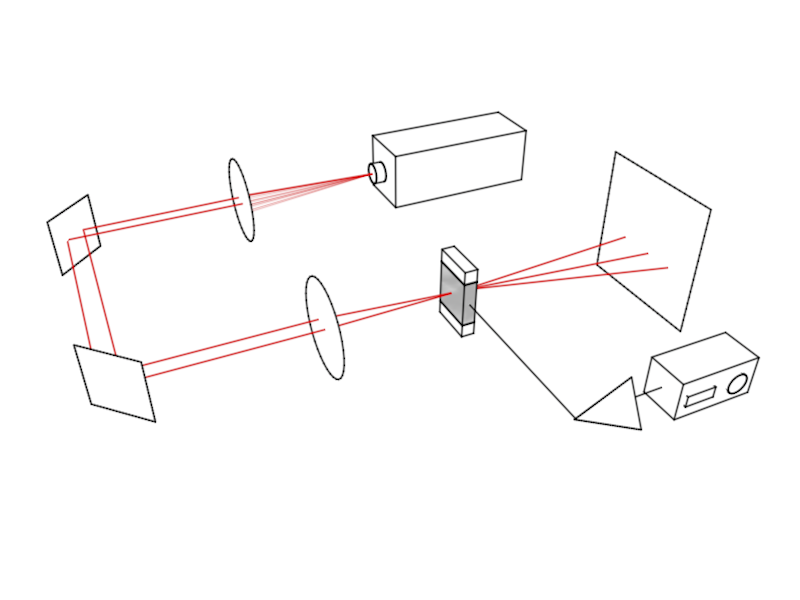
\includegraphics[width=\linewidth]{tegninger/tegning1.png}
    \caption{Opstilling til delforsøg 1.}
    \label{fig:opstilling1}
\end{figure}
\subsection{Delforsøg 2}
Til forskel fra delforsøg 1, placeres en switch pkt. 9, i mellem frekvens generatoren og forstærkeren på \cref{fig:opstilling2}. Skærmen pkt 6. Er brugt til at afskærme den ene stråle, hvorefter den anden stråle opsamles på en fotodetektor i pkt. 10. I praksis, er føleren på fotodetekteren meget lille, så der anvendes en linse til at fokusere beamen på detekteren. Ud over det, anvendes der også et oscialtorscop til at logge spændingen.
    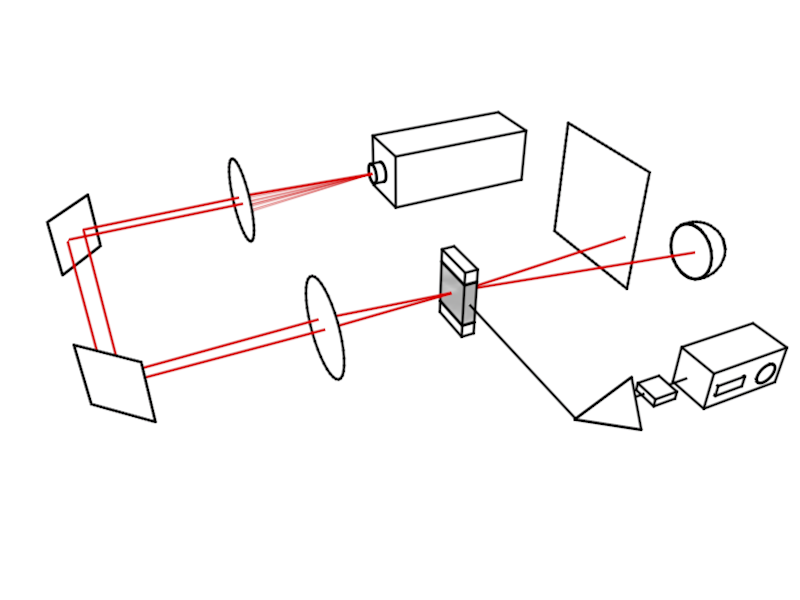
\includegraphics[width=\linewidth]{tegninger/tegning2.png}
    \caption{Opstilling til delforsøg 2.}
    \label{fig:opstilling2}
\end{figure}

\end{document}
